%%%%%%%%%%%%%%%%%%%%%%%%%%%%%%%%%%%%%%%%%%%%%%%%%%%%%%%%%%%%%%%%%%%%%%%%%%%%%%%%
% data_set.tex:
%%%%%%%%%%%%%%%%%%%%%%%%%%%%%%%%%%%%%%%%%%%%%%%%%%%%%%%%%%%%%%%%%%%%%%%%%%%%%%%%
\chapter{Background Estimation}
\label{sec:backgroundEstimation}
%%%%%%%%%%%%%%%%%%%%%%%%%%%%%%%%%%%%%%%%%%%%%%%%%%%%%%%%%%%%%%%%%%%%%%%%%%%%%%%%
Data used in the $ee$- and $\mu\mu$-channel searches contained events produced by ST backgrounds.  
Applying the event selection described in Chapter \ref{sec:event_selection_chapter} to data reduced 
the number of background events found in the $\Mlljj$ distribution, but did not eliminate them.  The 
contributions of ST backgrounds to the $\Mlljj$ distribution found in data was estimated using procedures 
described in this chapter.


\section{Top Quark Background}
\label{sec:topQrkBkgnds}
One of the two largest backgrounds in the \WR and \nul search was ST processes that produced at least 
one top quark, like top quark $\plus$ $W$ boson production (top+W, Figure \ref{fig:singleTopDiags}), 
and top anti-top quark pair production ($\ttbar$, Figure \ref{fig:ttbarDiag}).  Top 
quarks decay to a $W$ boson and bottom (b) quark, which subsequently decay to leptons and hadrons.  
Based on lepton universality in $W$ boson and b quark decays, events with top (or anti-top) quarks produce 
the $e\mu jj$ final state ($e\mu$-channel) at twice the rate of the $eejj$ or $\mu\mu jj$ final states.  At leading order 
in the weak coupling constant, the \WR cannot decay through a \nul to the $e\mu jj$ final state, so $e\mu$-channel 
data events are essentially free of \WR signal.  This allowed $e\mu$-channel data events to be used to 
estimate the top quark contribution to the $\Meejj$ and $\Mmumujj$ distributions found in data.

\begin{figure}[h]
	\centering
	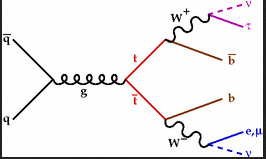
\includegraphics[width=0.7\textwidth]{figures/topAntiTopFeynDiagram.png}
	\caption{$\ttbar$ Feynman diagram \cite{ttbarDiagram}.}
	\label{fig:ttbarDiag}
\end{figure}

\begin{figure}[h]
	\centering
	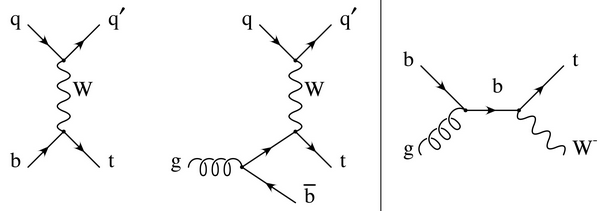
\includegraphics[width=0.7\textwidth]{figures/singleTopQuarkFeynDiagrams.png}
	\caption{Single top quark Feynman diagrams \cite{singleTopQrkDiagrams}.}
	\label{fig:singleTopDiags}
\end{figure}

Data events in the $e\mu$-channel were selected by a Level-1 trigger that required a track in at least one 
muon DT or CSC detector with $\pt > 16$ $\GeV$.  Events that passed the Level-1 selection were reconstructed 
if they passed the following electron and muon HLT selections:

\begin{itemize}
	\item A track reconstructed in the silicon tracker with $\pt > 30$ $\GeV$ and $|\eta| < 2.4$ was geometrically matched to 
		the muon detector hits that passed the L1 trigger.  Considering this set of muon detector hits and the matching 
		reconstructed track:
	\begin{itemize}
		\item A curve representing the muon trajectory through CMS was fitted to the reconstructed track and at least one 
			muon detector hit with $\chi^{2}/nDOF < 20$.
		\item In the plane perpendicular to the beam axis, the distance between the reconstructed track origin and its 
			reconstructed vertex was $< 1$ mm.
	\end{itemize}
	\item One ECAL SC was detected with $\Et > 30$ $\GeV$.
	\item For the SC:
	\begin{itemize}
		\item The ratio of hadronic energy in the HCAL tower behind the SC to the SC energy was $< 0.15$ in the barrel, and $< 0.1$ in the endcap.
		\item Ninety percent of the SC energy was measured in an $(\eta, \phi)$ region that is two crystals wide in $\eta$.
		\item For SCs in the barrel, a reconstructed track with hits in at least two pixel tracker layers extrapolated to the 
			SC centroid along the beam axis within 2.3 \cm, and extrapolated to the SC centroid in $(\eta_{SC}, \phi_{SC})$ within the 
			$(\eta, \phi)$ area of one ECAL crystal.
	\end{itemize}
\end{itemize}

The reconstructed $e\mu$ data events were filtered by the electron, muon, and jet selections described 
in Chapter \ref{sec:event_selection_chapter}, with the additional requirements that one selected lepton was a muon, the other was an electron, 
and at least one lepton had $\pt > 60$ $\GeV$.  Simulated ST background events were selected with the 
same online and offline requirements, and compared to the $e\mu$-channel data.  Top quark backgrounds 
produced the majority of events that passed the $e\mu$-channel selections, as shown in Figure \ref{fig:dataAndSimsInEMuChannel}.  

\begin{figure}[h]
	\centering
	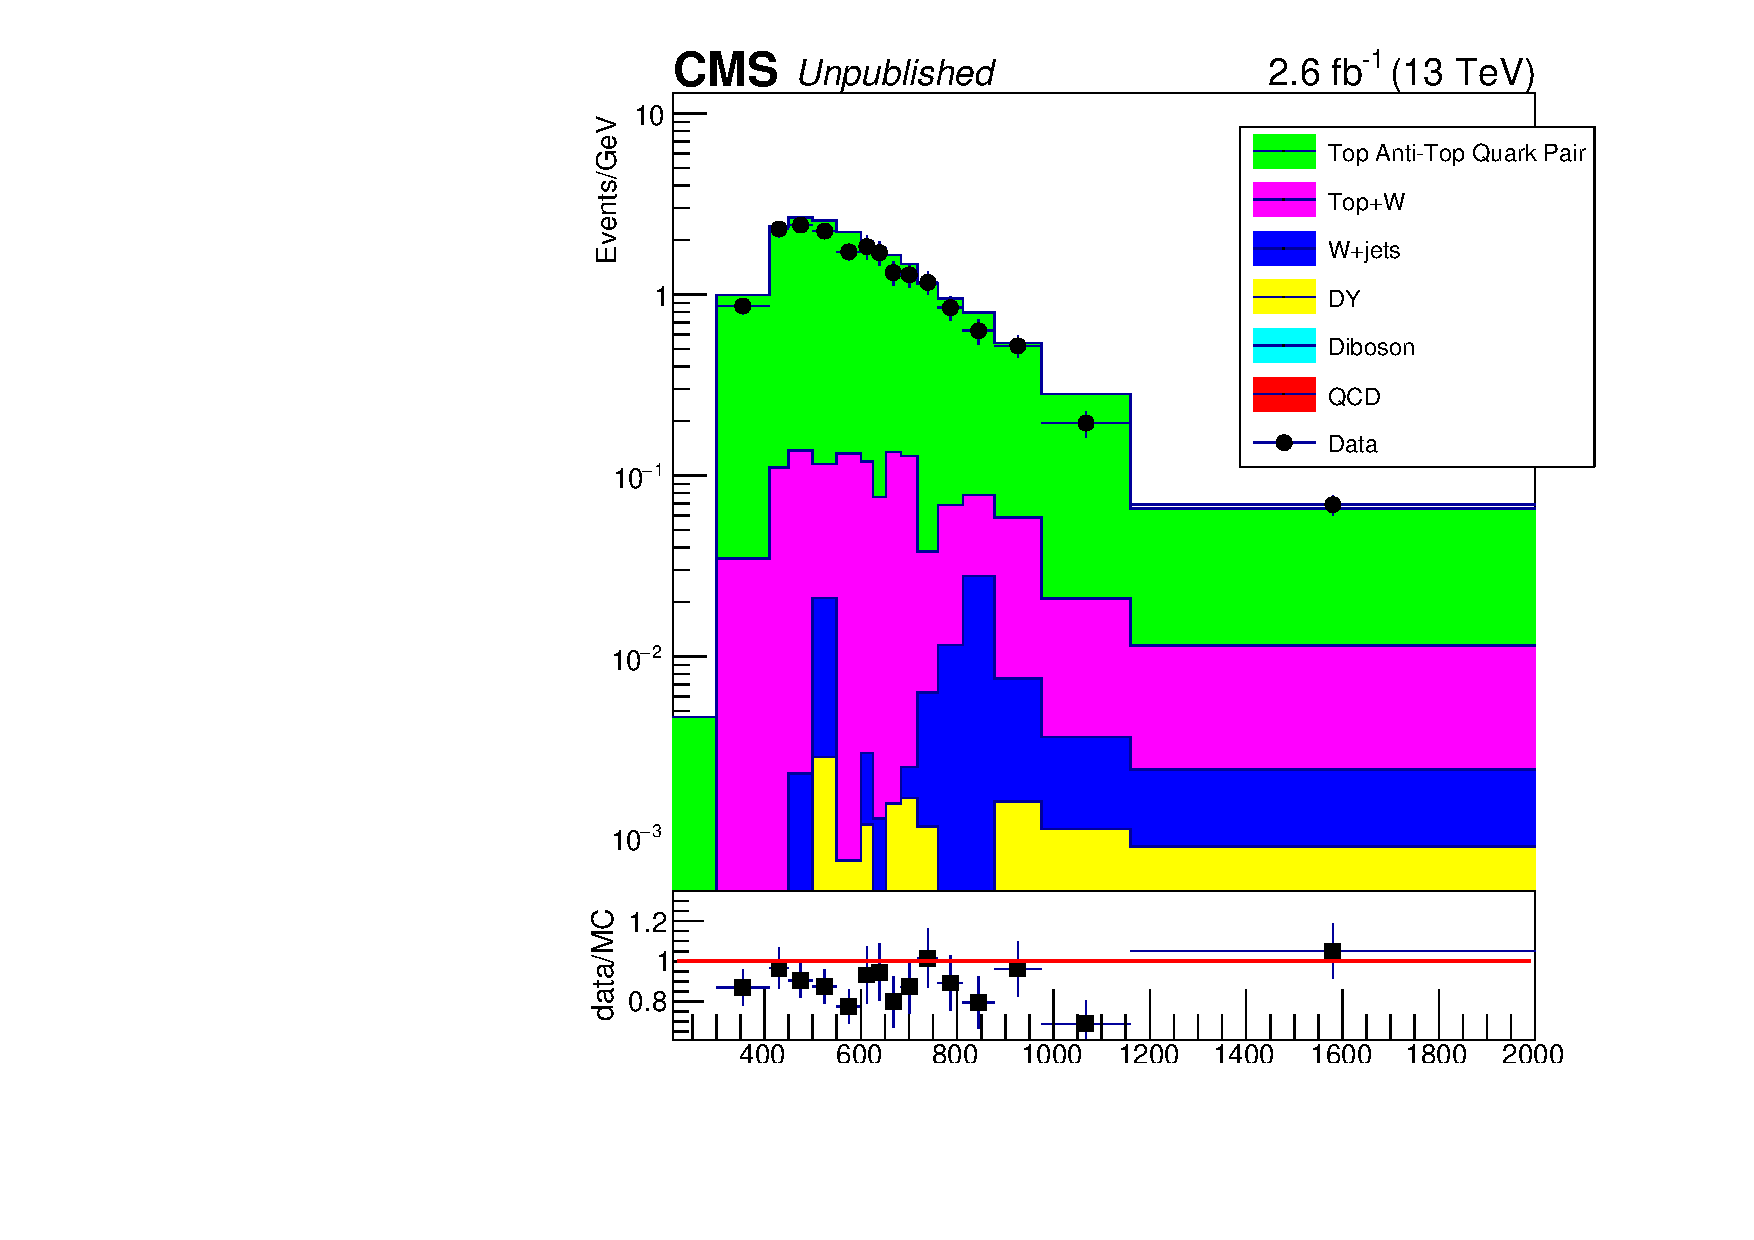
\includegraphics[width=0.7\textwidth]{figures/Mlljj_eMuChannel_log.pdf}
	\caption{The $\Mlljj$ distribution from data and simulated ST events that passed the $e\mu$ selection, excluding 
	the $\Mlljj > 600 \GeV$ cut.  The bin widths were variable, and their contents were normalized to the bin widths.}
	\label{fig:dataAndSimsInEMuChannel}
\end{figure}

The $\Memujj$ distribution found in data were used to represent the top quark background, and its shape was expected 
to be the same in the $\Meejj$ and $\Mmumujj$ distributions.  This expectation was tested using simulated 
top quark events.  Simulated events were selected using the $ee$-, $e\mu$-, and $\mu\mu$-channel requirements, and were used 
to produce $\Meejj$, $\Memujj$, and $\Mmumujj$ distributions.  The ratios of the binned distributions $\Meejj / \Memujj$ 
and $\Mmumujj / \Memujj$, shown in Figure \ref{fig:ttbarSFratios}, were consistent with constant values within 
the statistical uncertainty of each bin.  Each ratio was approximately independent of $\Mlljj$, which indicated that the $\Mlljj$ 
distribution shape in top quark events was the same in all three lepton channels.  Therefore, the shape of 
the $\Memujj$ distribution found in data represented the shape of the top quark background in the $\Meejj$ 
and $\Mmumujj$ distributions.

As the top quark background shape was the same in all lepton channels, the only difference between the top quark 
background in the $e\mu$-channel and either same flavor $\ell\ell$-channel was a difference in normalization.
This normalization difference was estimated using the invariant mass 
ratios, $\Mlljj / \Memujj$, obtained from simulated top quark events passing selections.  For each channel an average 
ratio, or normalization factor (NF), was calculated by integrating the $\Mlljj$ and $\Memujj$ distributions and 
dividing the integrals, $\int \Mlljj / \int \Memujj$.  The NF was 0.659 for the $\mu\mu$-channel, 
and 0.432 for the $ee$-channel.  These NFs differed from the expected value of 0.5 because the acceptance $\times$ 
selection efficiency of electrons was lower than that of muons.  Multiplying the $\Memujj$ distribution found in 
data by 0.659 (0.432) predicted the top quark contribution to the $\Mmumujj$ ($\Meejj$) distribution found in data.

The NFs were calculated using simulated events with $\Mlljj > 600$, but were dominated by events with $\Mlljj < 1500$ $\GeV$.  
As a result, an error entered the top quark background estimate that was proportional to the per-bin fluctuations 
of the $\Mlljj / \Memujj$ ratios around the NFs shown in Figure \ref{fig:ttbarSFratios}.  The impact of this error 
was covered by assigning a 10\% uncertainty to both NFs.  The contribution of non-top quark backgrounds to the $\Memujj$ 
distribution found in data, represented by simulated events in Figure \ref{fig:dataAndSimsInEMuChannel}, was more 
than one order of magnitude smaller than the NF uncertainty, so these backgrounds were not subtracted from 
the $e\mu$-channel data.

\begin{figure}[btp]
	\centering
	\subfigure{
		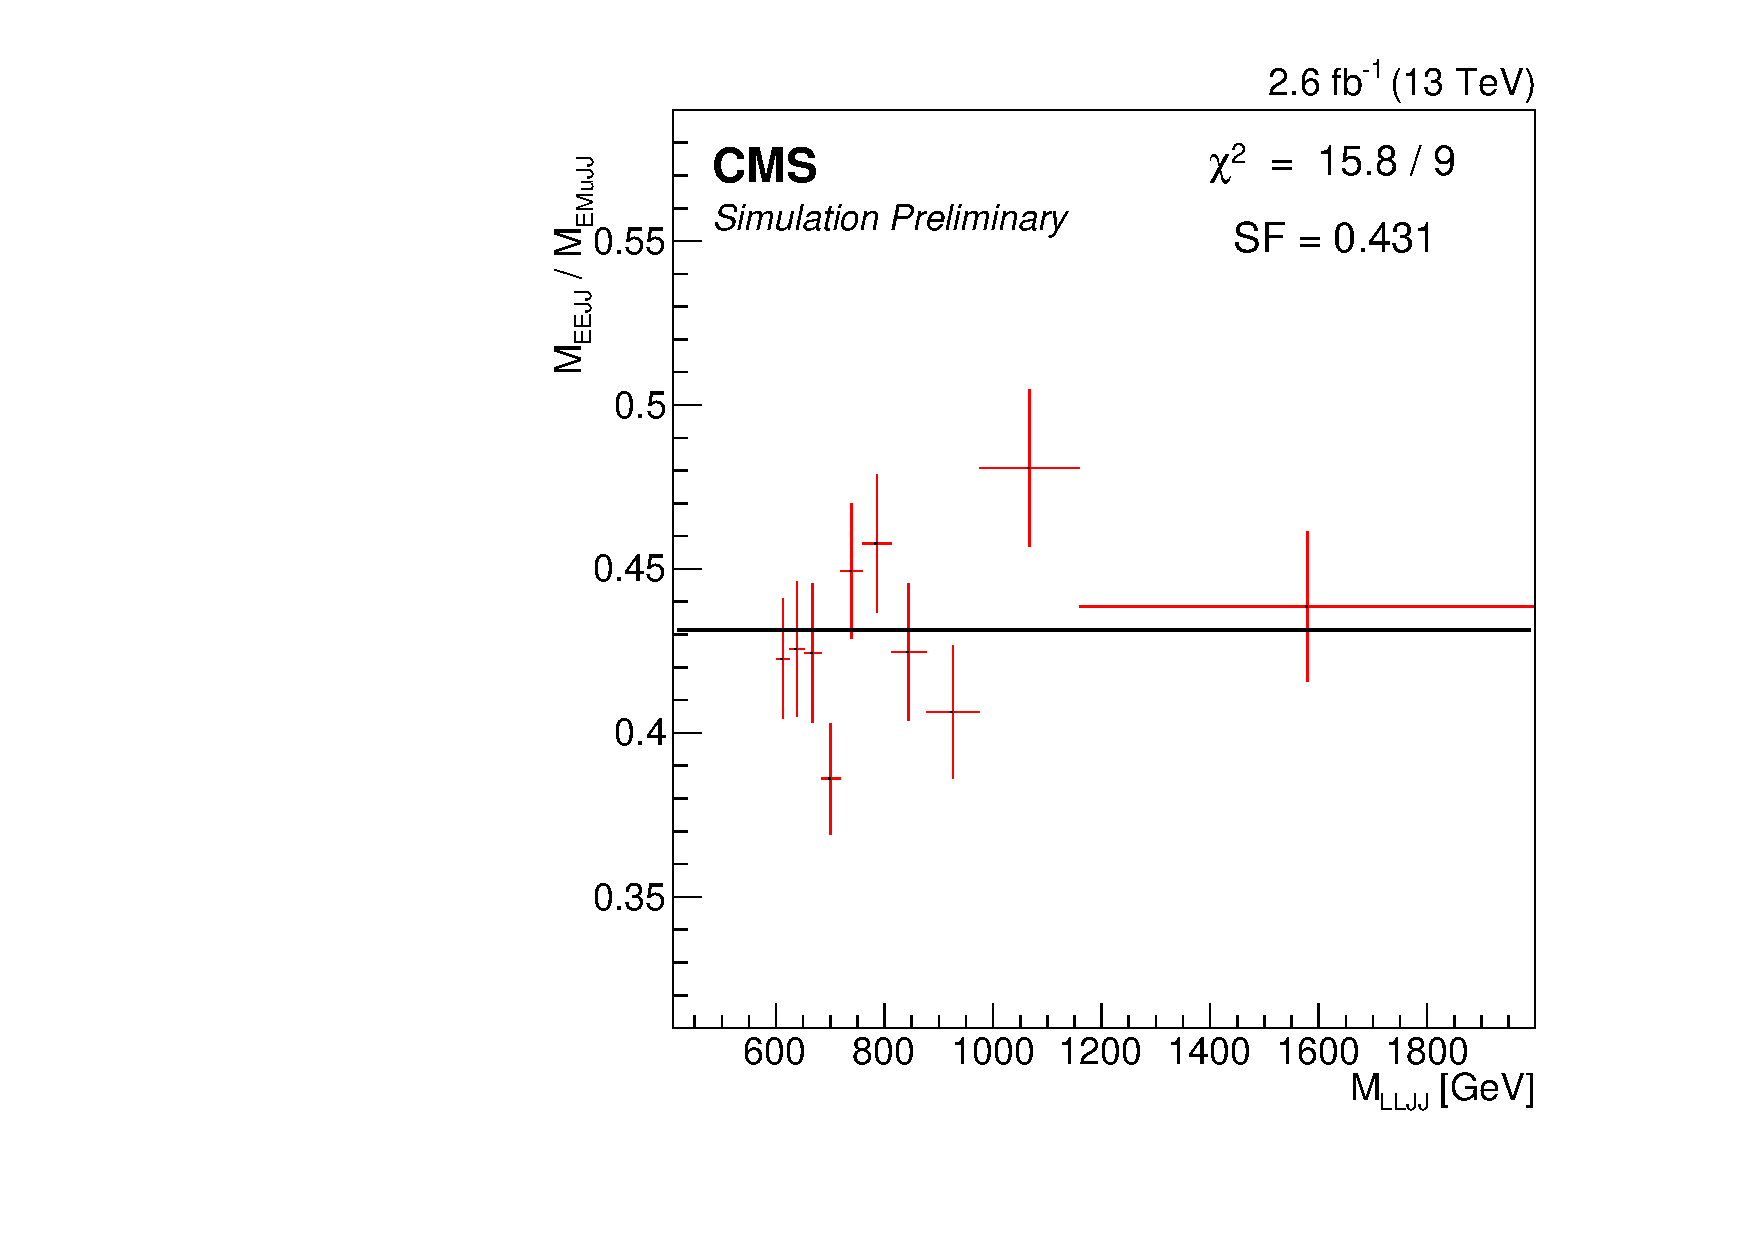
\includegraphics[width=0.45\textwidth]{figures/flavor_ratio_EE_variablebinwidth.pdf}
	}
	\subfigure{
		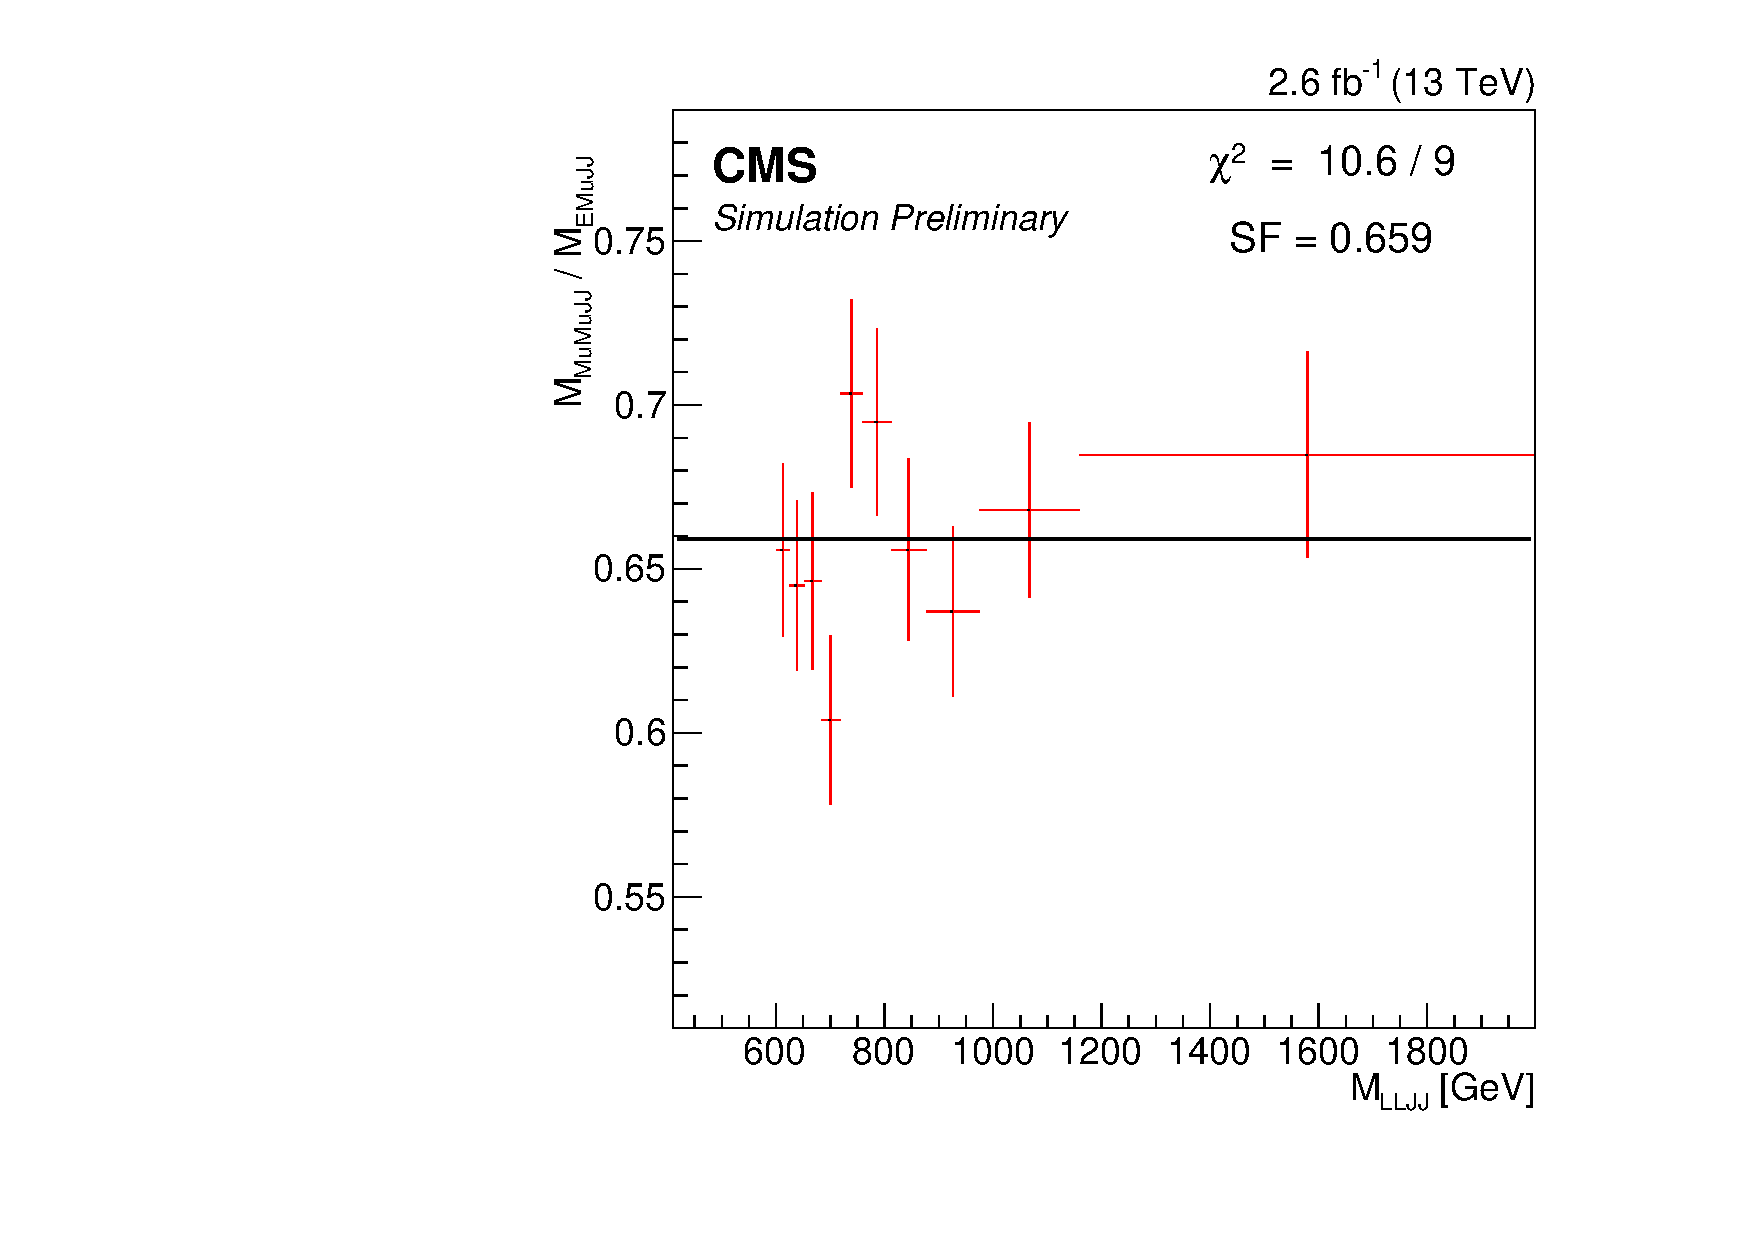
\includegraphics[width=0.45\textwidth]{figures/flavor_ratio_MuMu_variablebinwidth.pdf}
	}
	\label{fig:ttbarSFratios}
	\caption{The bin-by-bin ratio of the $\Mlljj$ and $\Memujj$ distributions from simulated top quark backgrounds, where 
		$\ell$ is an electron on the left, and a muon on the right.}
\end{figure}


\section{\DY Background}
\label{sec:dyBkgnd}
The second of the two largest backgrounds in the \WR and \nul search was the production and decay of a Z boson to 
a lepton pair in association with jets (\DY), $pp \rightarrow Z+jets \rightarrow \ell\ell+jets$.  The \DY 
background was estimated using simulated $\DY$+jets events selected with the $ee$- and $\mu\mu$-channel requirements 
described previously.  $\DY$+jets simulations were developed to model $\DY$+jets interactions observed in data, and 
mis-modelling in simulations lead to two discrepancies between $\DY$+jets simulations and data.

\subsection{\DY Normalization in $\Mlljj$}
\label{sec:dyNormInMlljj}
$\DY$+jets events were simulated using the \MADGRAPH generator at leading order in the electroweak and strong coupling 
constants, while $\DY$+jets events observed in data were produced at all orders in these coupling constants.  The 
simulated dataset contained more events than were expected in the 2.6 fb$^{-1}$ of data, so the simulated events were 
weighted to the integrated luminosity of data using an uncertain cross section $\times$ branching fraction calculated during 
simulations.  The cross section $\times$ branching fraction uncertainty was sensitive to the higher order electroweak 
and strong coupling corrections, and it created a discrepancy in the $\Mlljj$ distribution normalization between data 
and simulated events.

The magnitude of the normalization discrepancy in the $\Mlljj$ distribution was estimated 
using a $Z \rightarrow \ell\ell$ control region where data and simulated events were expected to agree.  Data and simulated 
$\DY$+jets events in the $ee$-channel control region were selected by a Level-1 trigger that required one ECAL SC with 
$\Et > 30$ $\GeV$ and $|\eta| < 2.1$.  Events that passed the Level-1 selection were used offline if they passed the 
following double electron HLT selections:

\begin{itemize}
	\item One SC was detected with $\Et > 30$ $\GeV$, and a second non-overlapping SC was detected with $\Et > 4$ $\GeV$.
	\item For the SC with $\Et > 30$ $\GeV$:
	\begin{itemize}
		\item The ratio of hadronic energy in the HCAL tower behind the SC to the SC energy was $< 0.055$ in the barrel, and 
			$< 0.07$ in the endcap.
		\item Ninety percent of the SC energy was measured in an $(\eta, \phi)$ region that was two crystals wide in $\eta$.
		\item A reconstructed track with hits in at least two pixel tracker layers was matched to the SC, and extrapolated to the SC 
			centroid along the beam axis within 1 cm, and extrapolated to the SC centroid in $(\eta, \phi)$ within the $(\eta, \phi)$ 
			area of $\frac{1}{2}$ an ECAL crystal.  In addition, the SC energy and track momentum cannot differ by more than 50\%.
		\item In a cone of radius $\Delta R =$ 0.3 centered on the SC:
		\begin{itemize}
			\item The fraction of the total ECAL energy in the cone not associated with the SC was $< 0.225$ in the barrel, and 
				$< 0.121$ in the endcap.
			\item The total HCAL energy in the cone divided by the SC energy is $< 0.155$ in the barrel, and $< 0.16$ in the endcap.
		\end{itemize}
	\end{itemize}
\end{itemize}

Data and simulated events in the $\mu\mu$-channel control region were selected by a Level-1 trigger that required a track 
in at least one muon DT or CSC detector with $\pt > 20$ $\GeV$.  Events that passed the Level-1 selection were used offline 
if they passed the following single muon HLT selections:

\begin{itemize}
	\item A track reconstructed in the silicon tracker with $\pt > 22$ $\GeV$ and $|\eta| < 2.4$ was geometrically matched to 
		the muon detector hits that passed the L1 trigger.  Considering this set of muon detector hits and the matching reconstructed 
		track:
	\begin{itemize}
		\item A curve representing the muon trajectory through CMS was fitted to the reconstructed track and at least 
			one muon detector hit with $\chi^{2}/nDOF < 20$.
		\item In the plane perpendicular to the beam axis, the distance between the reconstructed track origin and its 
			reconstructed vertex was $< 1$ mm.
		\item In a cone of radius $\Delta R =$ 0.3 centered on the muon trajectory:
		\begin{itemize}
			\item The total ECAL energy in the cone divided by the momentum measured by the muon detectors is $< 0.11$ in 
				the barrel, and $< 0.08$ in the endcap.
			\item The total HCAL energy in the cone divided by the momentum measured by the muon detectors is $< 0.21$ in 
				the barrel, and $< 0.22$ in the endcap.
			\item The total $\pt$ of all silicon tracker tracks in the cone (excluding the muon track) divided by the 
				muon track $\pt$ is $< 0.09$.
		\end{itemize}
	\end{itemize}
\end{itemize}

Similar to the offline lepton and jet selections used in the \WR search and defined in Chapters \ref{sec:muonSelection}, \ref{sec:electronSelection}, 
and \ref{sec:jetSelection}, reconstructed events in both channels were required to have two leptons and two jets passing kinematic 
and ID selections.  However, looser lepton $\pt$ and $\Mll$ selections were used to select events in the $Z \rightarrow \ell\ell$ 
mass window.  The differences and similarities between the $Z \rightarrow \ell\ell$ control region and the \WR search selections 
are listed in Table \ref{tab:cutCompSignalRegAndZllReg}.

\begin{table}[h]
	\caption{The corrections and selections applied to events used in the \WR search, and events used to estimate the \DY 
	background normalization discrepancy.  \textbf{Differences} in \textbf{bold}. (energies and masses in $\GeV$)}
	\label{tab:cutCompSignalRegAndZllReg}
	\centering
	\begin{tabular}{c|c|c}
		Correction & \WR search region & $Z \rightarrow \ell\ell$ region \\  \hline
		lepton energy & applied & identical applied \\
		jet energy & applied & identical applied \\
		trigger selection efficiency & applied & applied (different values) \\
		lepton reco and selection efficiency & applied & identical applied \\	\hline
		Selection & \WR search region & $Z \rightarrow \ell\ell$ region \\  \hline
		jet $\pt$ and $\eta$ & $\pt > 40$, $|\eta| < 2.4$ & identical applied \\
		jet ID & applied & identical applied \\
		lepton-jet separation & $\Delta R > 0.4$ & identical applied \\
		lepton ID & applied & identical applied \\
		\textbf{lepton} $\pt$ \textbf{and} $\eta$ & $\pt > 60, 53$, both $|\eta| < 2.4$ & both $\pt > 35$, $|\eta| < 2.4$ \\
		\textbf{di-lepton mass} $\Mll$ & $> 200$ & $70 < \Mll < 110$ \\
		\textbf{di-lepton di-jet mass} $\Mlljj$ & $> 600$ & none applied \\	\hline
	\end{tabular}
\end{table}

Events in data and $\DY$+jets simulations passing the $Z \rightarrow \ell\ell$ selections were used to produce a $\Mll$ 
distribution.  In both lepton channels, the $\Mll$ distribution shape agreed between data and simulated events.  The 
normalization of the $\Mll$ distribution in data events exceeded that of simulated events by 15.7\% in the $ee$-channel, 
and 14.2\% in the $\mu\mu$-channel.  To correct this normalization discrepancy, the $\DY$ background predicted using 
simulated events was increased by $\sim$15\%.  The contamination of other ST backgrounds in selected data events was 
estimated using simulated background events selected with the requirements described above, and found to be $\sim$3\%.  
This was similar to the uncertainty on the $\sim$15\% correction discussed next, so other ST backgrounds were not subtracted 
from data.

Two additional simulated $\DY$+jets datasets were produced with different \MC generators, and used to estimate the uncertainty 
on the $\sim$15\% \DY background correction.  Events from data and all three simulated $\DY$+jets datasets were selected 
using the $Z \rightarrow \ell\ell$ selections without jet requirements.  The jet requirements were removed to compare data 
to simulations in a phase space where all three simulated datasets yielded a large number of events after selections.  Selected 
events were used to produce $\Mll$ distributions, and the difference in $\Mll$ normalization was calculated between data and each 
set of simulated events.  The largest difference was taken as the uncertainty on $\sim$15\%.  The uncertainty was 2.0\% in the 
$ee$-channel, and 1.0\% in the $\mu\mu$-channel.

\subsection{\DY Shape in $\Mlljj$}
\label{sec:dyShapeInMlljj}
In $\DY$+jets events from data or simulations, the Z production and decay was reconstructed as a vertex that was 
most often the primary vertex (PV), which was defined as the vertex with the highest $\sum \pt$ of all associated 
tracks in the event.  Selected reconstructed jets were required to have at least one charged hadron from the PV, and the partons 
radiated during the Z production and decay produced the majority of charged hadrons that traced back to the PV\footnote{The 
contamination of $Z \rightarrow \tau\tau$ in events with $ee$+jets or $\mu\mu$+jets final states was minimized by 
requiring two leptons with $\pt > 53$ $\GeV$.}.  $\DY$+jets events were simulated with up to 4 partons radiated from 
the $Z \rightarrow \ell\ell$ interaction, while $\DY$+jets events observed in data were produced with any number - 
0, 2, 6, etc. - of partons radiated from the $Z \rightarrow \ell\ell$ interaction.  The limit of 4 radiated partons 
in simulated events reduced the number of reconstructed jets that could pass the selections, and affected the energy 
of selected jets, as multiple partons could contribute to the same jet.  These jet modelling effects produced a discrepancy 
in the $\Mlljj$ distribution shape between data and simulated events.

The magnitude of the shape discrepancy in the $\Mlljj$ distribution was estimated 
using a low $\Mll$ control region where data and simulated events were expected to agree.  Events from data and all simulated ST 
backgrounds in the $ee$- and $\mu\mu$-channel low $\Mll$ control regions were selected using the electron and muon triggers described in 
Chapter \ref{sec:triggers}.  Events passing the trigger selections were required to have two energetic jets and leptons 
with $\Mlljj > 600$ $\GeV$, but $\Mll < 180$ $\GeV$.  Excluding the $\Mll$ requirement, the corrections and selections 
used in the low $\Mll$ control region were identical to those used in the \WR search region (Table \ref{tab:cutCompSignalRegAndZllReg}).  
Selected events in data and simulations were used to produce $\Mlljj$ distributions, and the $\sim$15\% increase was 
applied to simulated $\DY$+jets events.  The $\Mlljj$ distributions from data and simulated events shown in Figure 
\ref{fig:mlljjLowDileptonMassSideband} were compared, and the $\Mlljj$ shape discrepancy was estimated as the largest 
percentage difference between data and the total simulated background in any bin.  The shape discrepancy magnitude was 
conservatively estimated to be 40\% in both lepton channels, constant versus $\Mlljj$.  When calculating results the 
40\% uncertainty was applied to the expected number of \DY events.

\begin{figure}[btp]
\centering
\subfigure{
  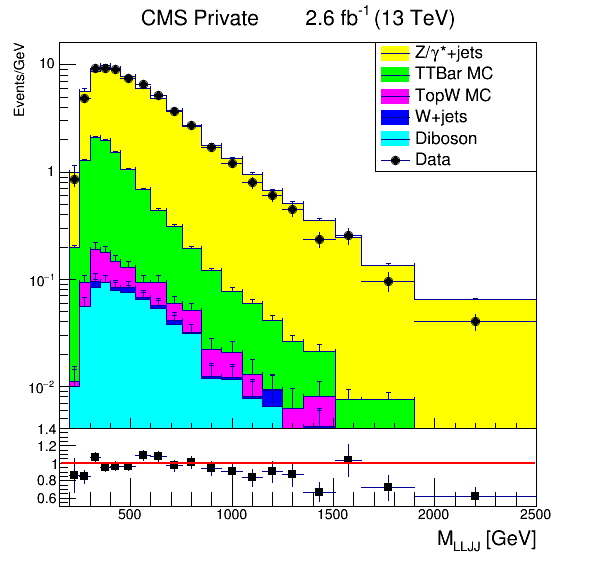
\includegraphics[width=0.45\textwidth]{figures/Mlljj_eeChnl_lowMllCR.png}
}
\subfigure{
  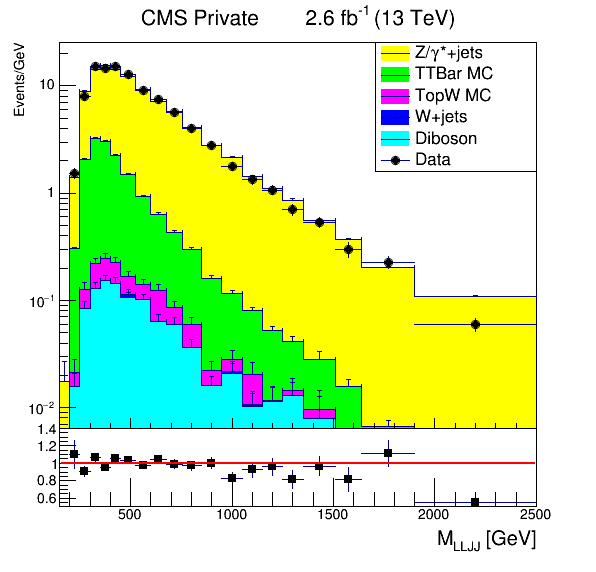
\includegraphics[width=0.45\textwidth]{figures/Mlljj_mumuChnl_lowMllCR.png}
}
\caption{The $\Mlljj$ distribution from data and simulated ST background events that passed the low $\Mll$ region selection, with 
	the $ee$- ($\mu\mu$-) channel on the left (right).  The bin widths are variable, and the bin contents are normalized to their widths.}
\label{fig:mlljjLowDileptonMassSideband}
\end{figure}

The $\DY$+jets simulation was produced at leading order in the strong coupling constant, and it was studied if the 40\% 
uncertainty assigned to the \DY background could be reduced by simulating higher order strong interactions.  $\DY$+jets 
events were simulated at next-to-leading order in the strong coupling constant, and were selected using the low $\Mll$ 
control region requirements.  Using the higher order simulation did not reduce the 40\% uncertainty, as shown in Figure 
\ref{fig:mlljjLowDileptonMassSidebandAMCNLO}.  The higher order simulation was limited by a lack of events with $\Mlljj > 600$ 
$\GeV$.  Relative to the leading order $\DY$+jets simulation, the higher order simulation had a factor of $\sim$3 fewer 
events with $\Mlljj > 600$ $\GeV$, and a factor of $\sim$10 fewer events with $\Mlljj > 1$ $\TeV$.

\begin{figure}[btp]
\centering
\subfigure{
  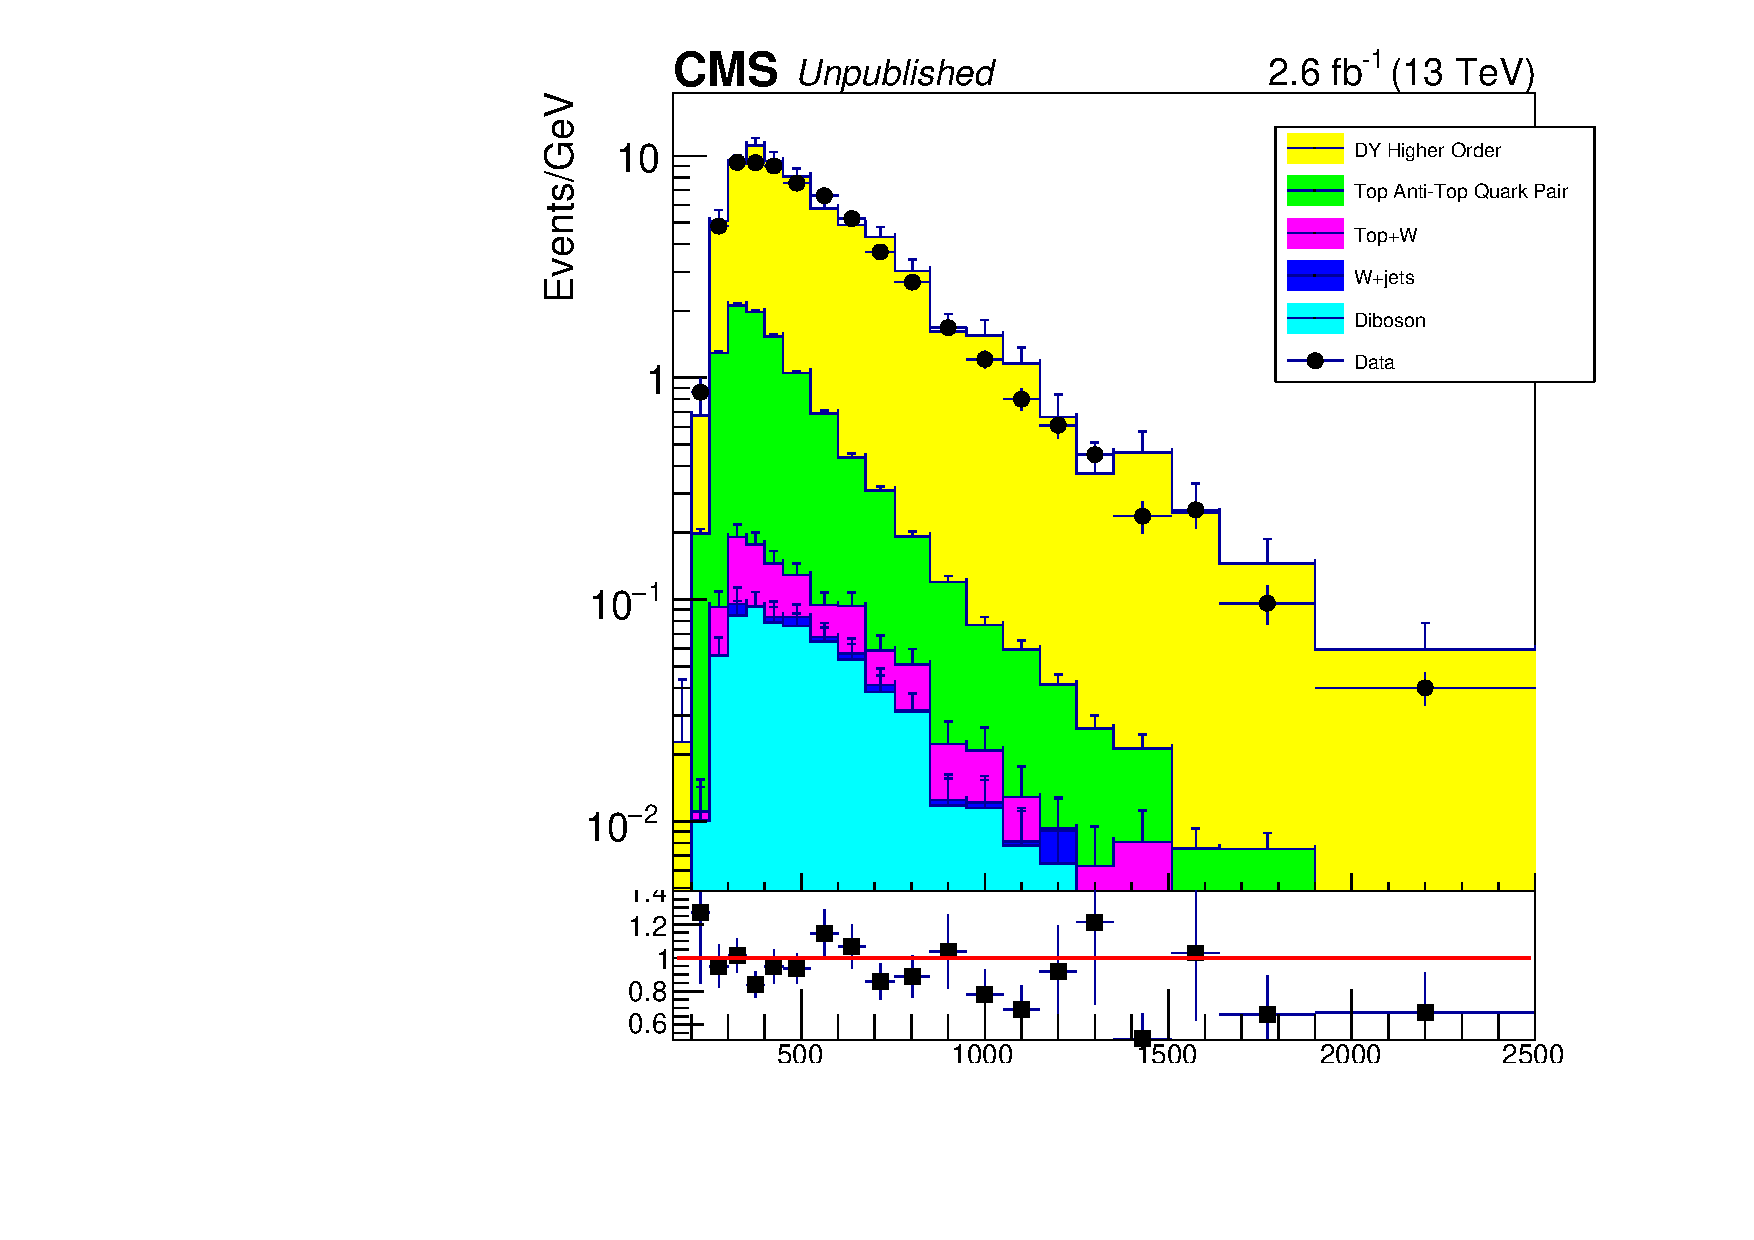
\includegraphics[width=0.45\textwidth]{figures/Mlljj_eeChnl_lowMllCR_AMCNLO.pdf}
}
\subfigure{
  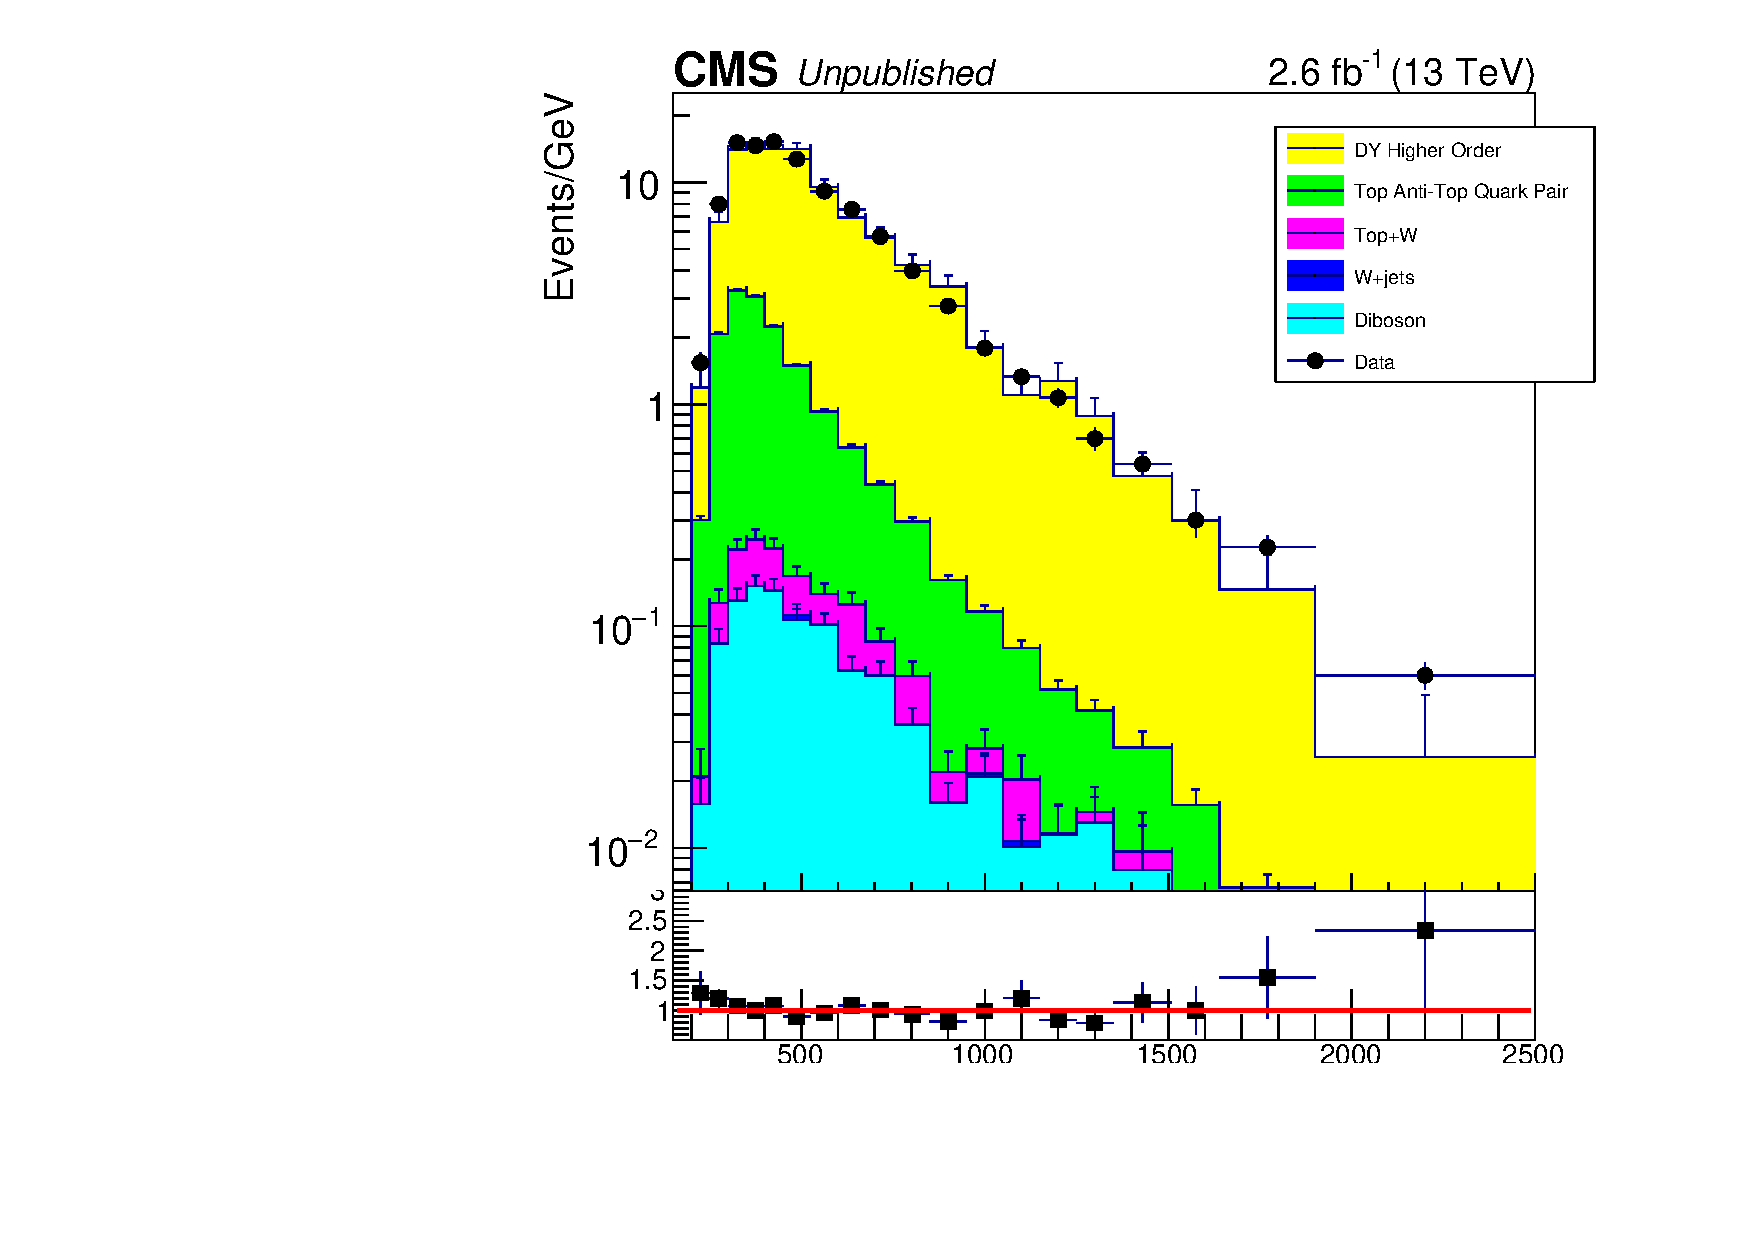
\includegraphics[width=0.45\textwidth]{figures/Mlljj_mumuChnl_lowMllCR_AMCNLO.pdf}
}
\caption{The $\Mlljj$ distribution from data and simulated ST events that passed the $\Mll < 180 \GeV$ selection, the 
		$ee$ ($\mu\mu$) channel on the left (right).  The bin contents are normalized to their widths.  Jet production 
	in \DY events was simulated at a higher order relative to the default \DY dataset.}
\label{fig:mlljjLowDileptonMassSidebandAMCNLO}
\end{figure}

The low $\Mlljj$ control region was used to validate the $\sim$15\% correction applied, and 40\% uncertainty assigned to 
the estimated \DY background.  In this control region, events from data and simulations of all ST backgrounds were selected 
using the \WR search requirements (Table \ref{tab:cutCompSignalRegAndZllReg}), but with $\Mlljj < 600 \GeV$.  Selected 
data and simulated events were used to make an $\Mll$ distribution, and the simulated \DY background was increased by $\sim$15\%.  
Comparing the $\Mll$ distributions found in data and simulations, shown in Figure \ref{fig:mllInLowMlljjSideband}, indicated 
that the $\sim$15\% \DY correction brought data and simulations into better agreement.  In addition, the comparison showed 
that the 40\% \DY normalization uncertainty was not too conservative, as the disagreement between data and simulated 
backgrounds approached 40\% in several bins.

\begin{figure}[btp]
\centering
\subfigure{
  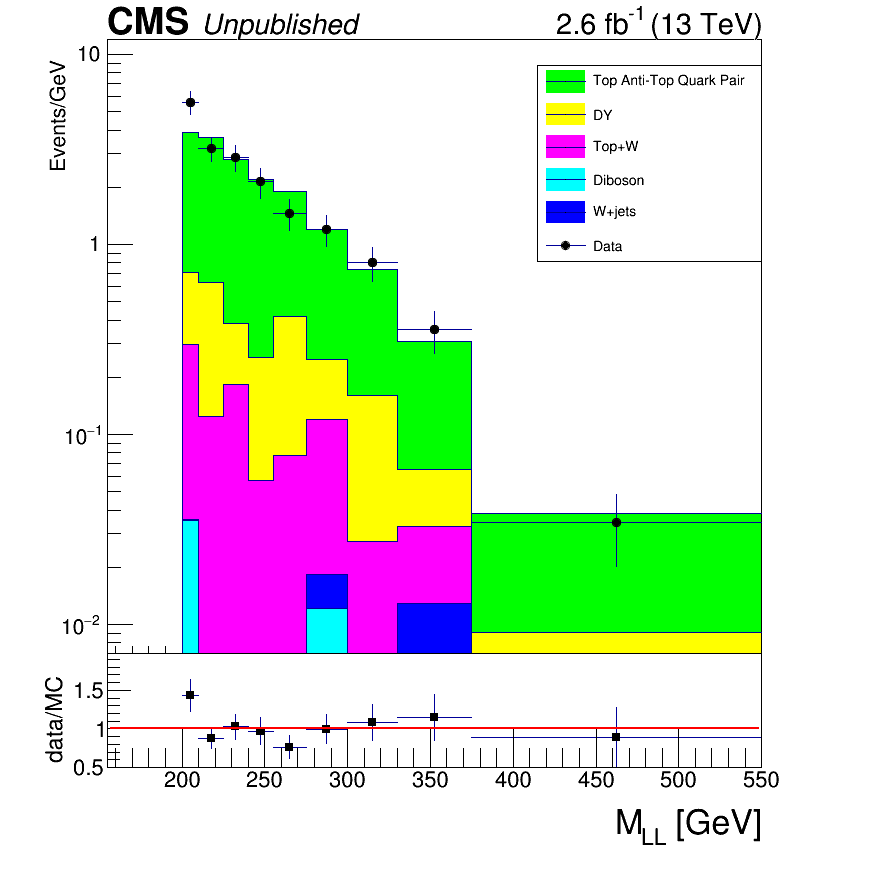
\includegraphics[width=0.45\textwidth]{figures/Mll_eeChnl_lowMlljjCR.png}
}
\subfigure{
  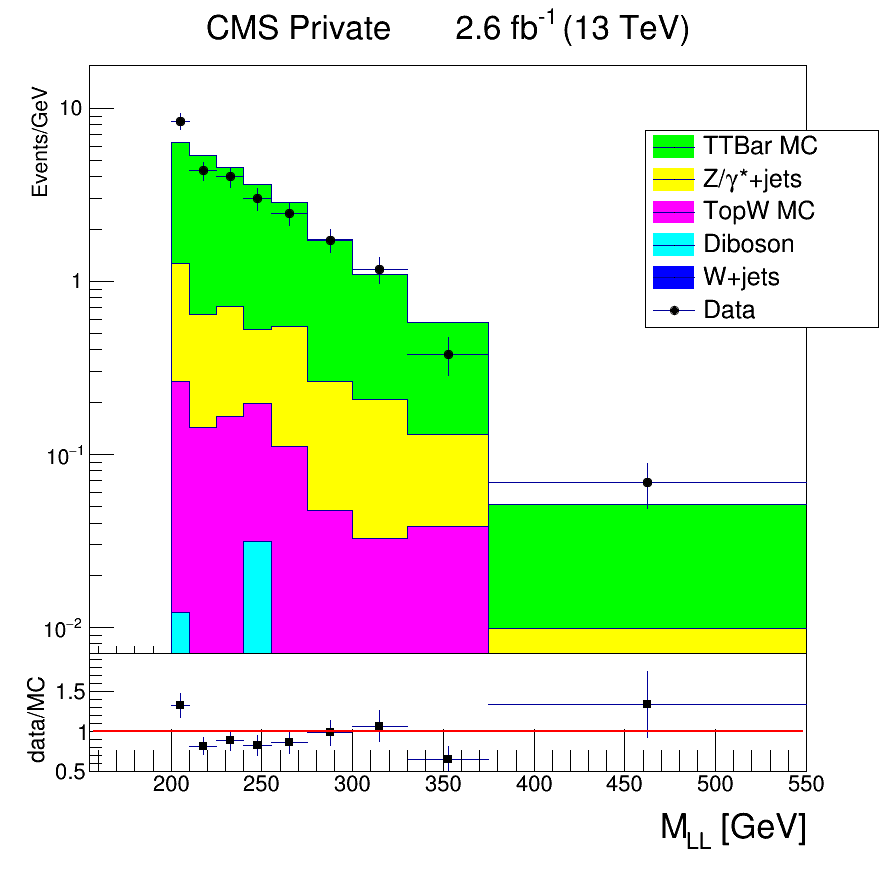
\includegraphics[width=0.45\textwidth]{figures/Mll_mumuChnl_lowMlljjCR.png}
}
\caption{$\Mll$ for data and simulations of all ST backgrounds in the $\Mlljj < 600\GeV$ control region.  The 
$ee$ ($\mu\mu$) channel was on the left (right).}
\label{fig:mllInLowMlljjSideband}
\end{figure}

\subsection{\DY Background Estimate}
The \DY contribution to the $\Mlljj$ distribution found in data was estimated by selecting simulated \DY events with the 
selections described in Chapter \ref{sec:event_selection_chapter}.  The weight of each selected event was multiplied by 1.157 
in the $ee$-channel, and by 1.142 in the $\mu\mu$-channel.  When calculating results a 40\% uncertainty was assigned to the 
estimated number of \DY events.


\section{Diboson and W+jets Backgrounds}
\label{sec:dibosonAndWJetsBkgnds}
The production of diboson (WW, WZ, ZZ), and single W bosons with jets (W+jets) yielded events where two charged leptons and 
jets were reconstructed.  The diboson and W+jets contributions to the $\Mlljj$ distribution found in data was estimated by 
selecting simulated diboson and W+jets events with the requirements described in Chapter \ref{sec:event_selection_chapter}.  
The result, shown in Figure \ref{fig:allExpectedBkgnds}, was that diboson and W+jets backgrounds were small compared to 
\DY and top quark backgrounds, and concentrated in the region $\Mlljj < 2000$ $\GeV$ where a \WR boson was excluded by 
previous searches.  Based on their small contributions, the estimated diboson and W+jets backgrounds were neglected when c
alculating results.

\begin{figure}[h]
	\centering
	\subfigure{
		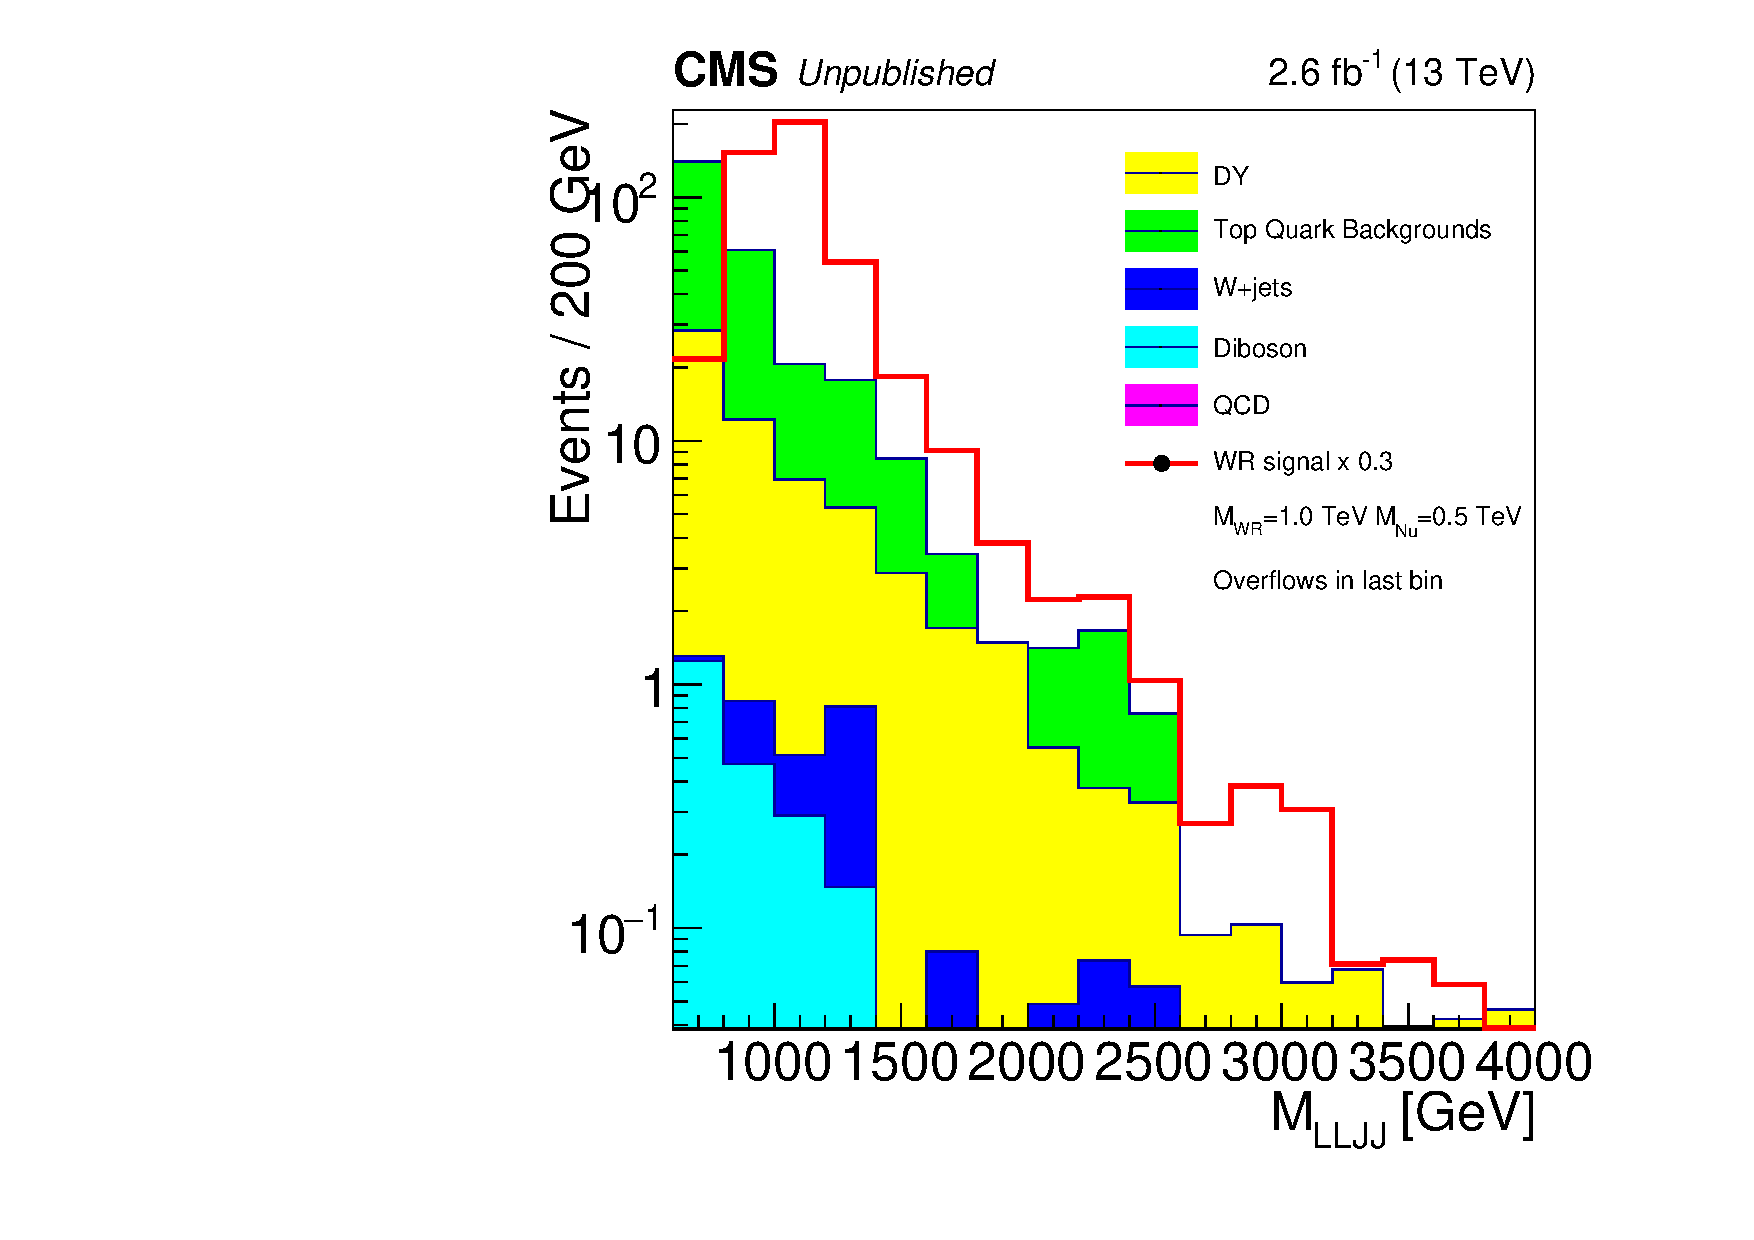
\includegraphics[width=0.45\textwidth]{figures/useOfLLJJMassAsFigureOfMerit.pdf}
	}
	\subfigure{
		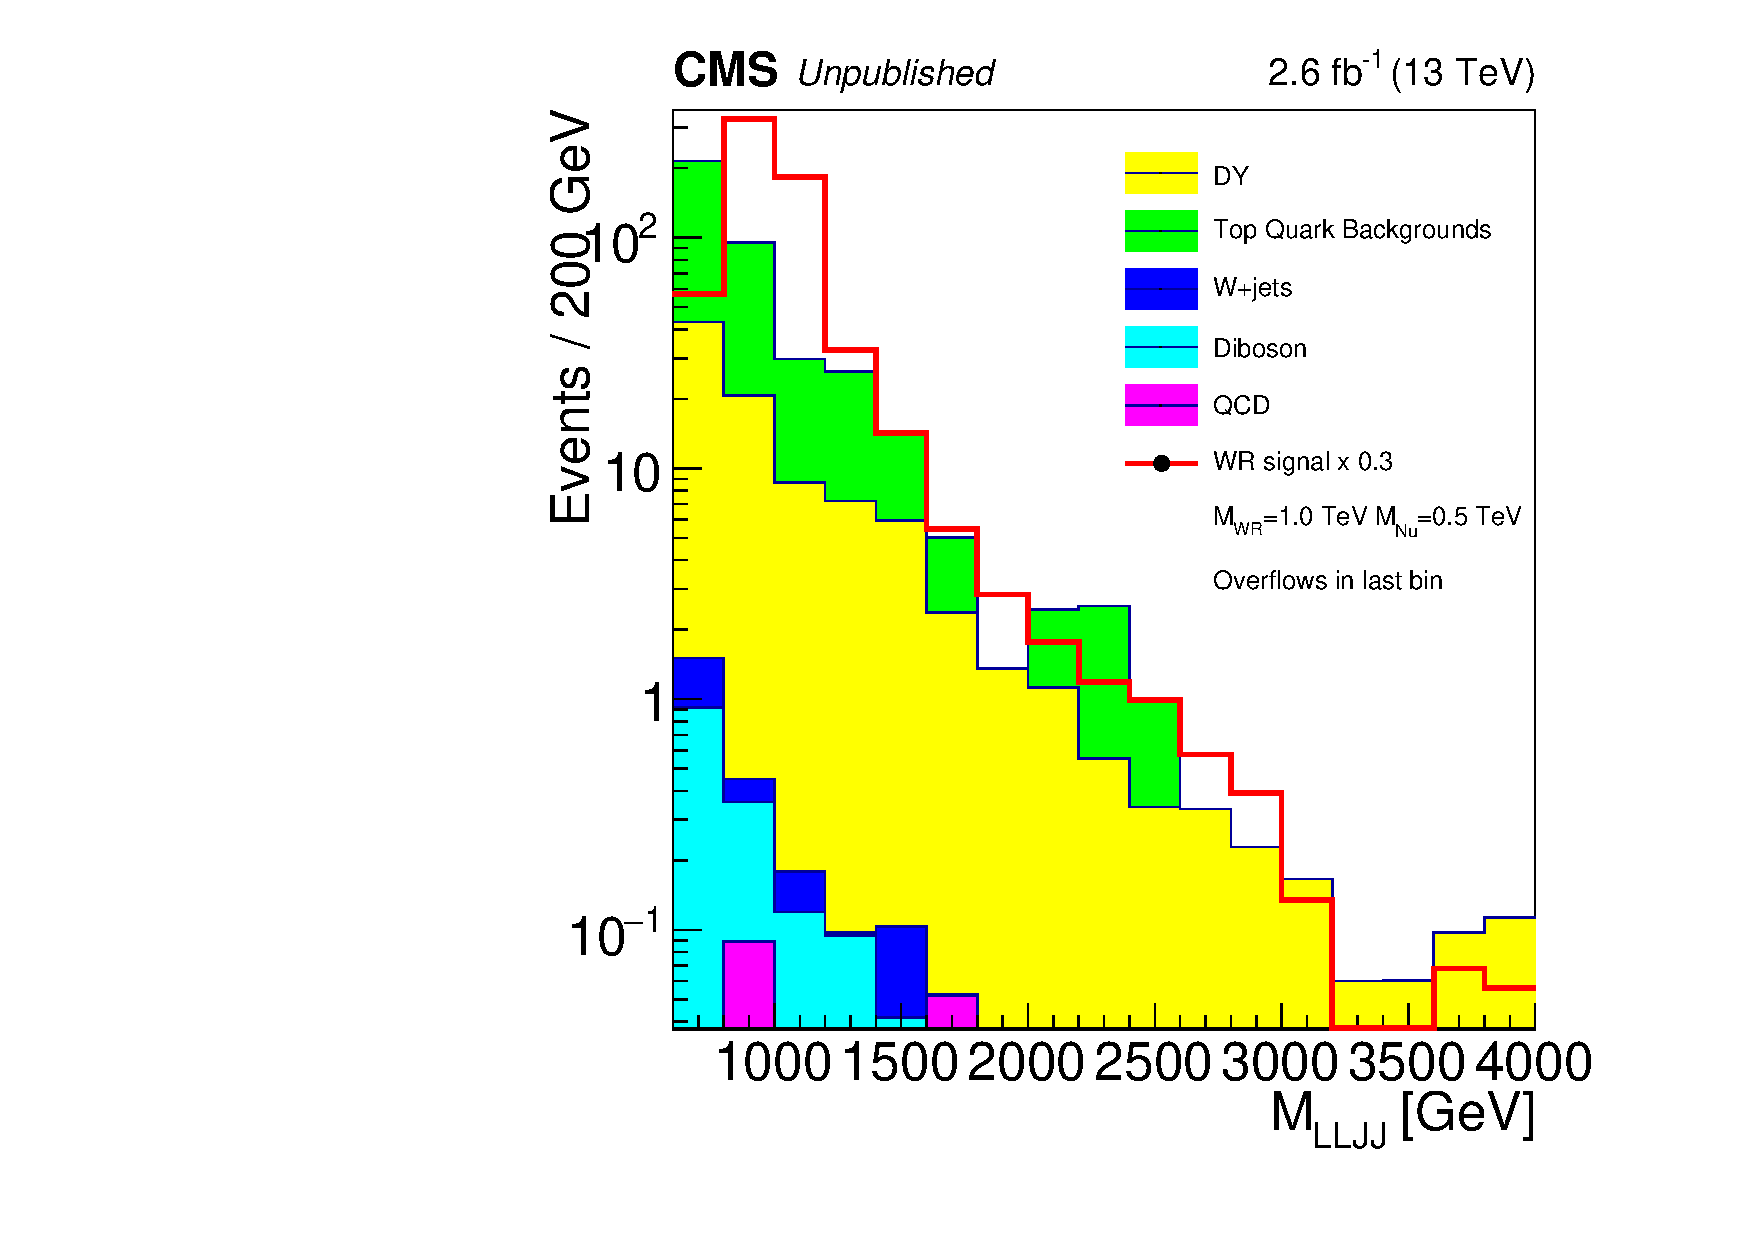
\includegraphics[width=0.45\textwidth]{figures/Mlljj_mumuChnl_signalRegionNoData.pdf}
	}
	\label{fig:allExpectedBkgnds}
	\caption{The $\Mlljj$ distributions from simulated \DY, diboson, W+jets backgrounds, and the top quark and QCD backgrounds estimated from 
		data. The normalization of the \WR $\Mlljj$ distribution was scaled down by 70\% to facilitate comparisons between expected 
		signal and backgrounds.  The $ee$ ($\mu\mu$) channel was shown on the left (right).}
\end{figure}


\section{QCD Background}
\label{sec:qcdBkgnd}
QCD multi-jet production yielded events where two charged leptons and jets were reconstructed.  In those events, two real 
jets were incorrectly reconstructed and identified as charged leptons.  The QCD multi-jet contribution to the $\Mlljj$ 
distribution found in data was estimated by selecting events in data with loose lepton ID requirements, then weighting selected 
events by the probability for selected leptons to pass the default (tight) lepton ID reuiqrements.  Data events were selected 
with the requirements described in Chapter \ref{sec:event_selection_chapter}, but with the following (looser) lepton ID 
requirements:

\begin{itemize}
	\item \textbf{Muons}
	\item The silicon tracker track was reconstructed from at least 1 hit in the silicon pixel detector, and at least 5 hits in the 
		entire tracker.
	\item The fitted track representing the estimated muon trajectory through all of CMS originated at a 
		point that was within 2 (5) mm of the muon's reconstructed vertex in the $x-y$ plane ($z$ axis). 
\end{itemize}

\begin{itemize}
	\item \textbf{Electrons}
	\item At least 90\% of the SC energy was measured in a region 2 crystals wide in $\eta$.
	\item The ratio of hadronic energy in the HCAL tower behind the SC to the SC energy was $< 0.15$ 
		in the barrel, and $< 0.10$ in the endcap.
	\item The electron track missed 1 or fewer layers in the silicon pixel or inner silicon strip detectors.
	\item The electron track origin and its reconstructed vertex were separated by a small distance in the $x-y$ plane, 
		$\Delta_{xy} < 0.2$ mm in the tracker barrel, and $\Delta_{xy} < 0.5$ mm in the tracker endcap.
\end{itemize}

Events were not selected if one or more reconstructed leptons passed the default (tighter) lepton ID selections, as these 
events likely had one or more real leptons.  In selected events, the $\Et$ or $\pt$, and $\eta$ of the two selected leptons 
were used to calculate a probability for both leptons to pass the default lepton ID selections.  The probability was calculated 
using empirical formulas for electrons and muons derived from data, and each selected event was weighted by its probability.  
The contribution of weighted events, representing the QCD background, to the $\Mlljj$ distribution found in data is shown in 
Figure \ref{fig:allExpectedBkgnds}, and was negligible compared to other ST backgrounds.  Based on its small contribution, the 
QCD background was ignored when calculating results.


%%%%%%%%%%%%%%%%%%%%%%%%%%%%%%%%%%%%%%%%%%%%%%%%%%%%%%%%%%%%%%%%%%%%%%%%%%%%%%%%
